\documentclass{report}
% Packages
\usepackage[utf8]{inputenc}          % setting default encoding
\usepackage[T1]{fontenc}             % setting default encoding format
\usepackage[ngerman]{babel}          % german language
\usepackage[german=quotes]{csquotes} % correct quoting using \enquote{}
%\usepackage[english]{babel}         % english language
%\usepackage{csquotes}               % correct quoting using \enquote{}

\usepackage[backend=biber, autocite=inline, style=ieee]{biblatex}
\usepackage{graphicx}                % various graphics formats
\usepackage[german]{varioref}        % nicer references using \vref
\usepackage[hidelinks]{hyperref}     % for links
\usepackage{lmodern}                 % Setting default font #
\usepackage{acronym}                 % Package for acronyms
\usepackage{scrlayer-scrpage}        % Package for header customization
\usepackage{booktabs}                % nicer tabs
\usepackage{caption}                 % better captions
\usepackage{tabto}                   % to intend tabs
\usepackage{tabularx}                % useful for many tab operations
\usepackage{amsmath,amssymb,amsfonts}% math packages
\usepackage{tocloft}                 % redefine table of contents
\usepackage{makeidx}                 % used for making the index
\usepackage{listings}                % for coding
\usepackage{color}                   % color for code
\usepackage{algpseudocode}           % for algorithmetic pseudocode
\usepackage{algorithm}               % for algorithms
\usepackage{algorithmicx}




% Page Layout

\oddsidemargin=0mm                   % Sets the left margin of odd pages to zero 
\evensidemargin=0mm                  % Sets the left margin of even pages to zero
\textwidth=159mm                     % sets the width of the text (max)
\textheight=251mm                    % sets the height of the text (max)
\topmargin=-18mm                     % Sets the top margin
\footheight=15mm                     % Sets the available height for the footer


\makeindex                           % start of index (note: don't forget to reference)

\addbibresource{bibliography.bib}    % add biblatex file
\DefineBibliographyStrings{ngerman}{andothers = {{et\,al\adddot}},}  
 % set language of biblatex file to german

% !TEX root = master.tex

% Definitions and Commands

\newcommand{\TitelDerArbeit}[1]{\def\DerTitelDerArbeit{#1}\hypersetup{pdftitle={#1}}}
\newcommand{\AutorDerArbeit}[1]{\def\DerAutorDerArbeit{#1}\hypersetup{pdfauthor={#1}}}
\newcommand{\Firma}[1]{\def\DerNameDerFirma{#1}}
\newcommand{\Hochschule}[1]{\def\DieHochschule{#1}}
\newcommand{\Kurs}[1]{\def\DieKursbezeichnung{#1}}
\newcommand{\Abteilung}[1]{\def\DerNameDerAbteilung{#1}}
\newcommand{\Studiengangsleiter}[1]{\def\DerStudiengangsleiter{#1}}
\newcommand{\WissBetreuer}[1]{\def\DerWissBetreuer{#1}}
\newcommand{\FirmenBetreuer}[1]{\def\DerFirmenBetreuer{#1}}
\newcommand{\Bearbeitungszeitraum}[1]{\def\DerBearbeitungszeitraum{#1}}
\newcommand{\Abgabedatum}[1]{\def\DasAbgabedatum{#1}}
\newcommand{\Matrikelnummer}[1]{\def\DieMatrikelnummer{#1}}
\newcommand{\Studienrichtung}[1]{\def\DieStudienrichtung{#1}}
\newcommand{\ArtDerArbeit}[1]{\def\DieArtDerArbeit{#1}}
\newcommand{\Bearbeitungszeit}[1]{\def\DieBearbeitungszeit{#1}}
\newcommand{\Literaturverzeichnis}{Literaturverzeichnis}
\newcommand{\SignatureAndDate}[1]{
    \par\noindent\makebox[5.5cm]{\hrulefill}  \hfill\makebox[5.5cm]{\hrulefill}
    \par\noindent\makebox[5.5cm][l]{Ort, Datum}      \hfill\makebox[5.5cm][l]{#1}
}

% Shortcuts for often used methods

\newcommand{\NN}{{\mathbb{N}}}

% Renamed commands



% Listings
%\renewcommand{\lstlistingname}{Quelltext}
%\renewcommand{\lstlistlistingname}{Quelltextverzeichnis}
%\lstset{
%  numbers=left,
%  numberstyle=\tiny,
%  captionpos=b,
%  basicstyle=\ttfamily\small
%}

\newcommand{\settingBibFootnoteCite}{
%\setlength{\bibparsep}{\parskip}
% Add some space between biblatex entries in the bibliography
\addbibresource{bibliography.bib}
% Add file bibliography.bib as biblatex resource
\DefineBibliographyStrings{ngerman}
% Change language of bib file to german
}

\newcommand{\setTitlePage}{
  % !TEX root =  master.tex
\begin{titlepage}
			\begin{center}
				\rule[0.5cm]{150mm}{0.2mm}
			\end{center}
			\hspace*{0.5cm}	
			
\includegraphics[scale=0.2]{./img/Firmenlogo.jpg} \hfill
			
\includegraphics[scale=0.09]{./img/DHBW-Logo.jpg} 
			\hspace*{0.3cm}
		\vspace{5cm}
		\begin{center}
		{\textbf{\Large{}\DerTitelDerArbeit}} \\[1.5cm]
		{\textbf{\large{}Studiengang Informatik}}\\[1cm]
		{\large{}\DieHochschule}\\[1.5cm]
\begin{minipage}{\textwidth}
		\centering
		{\textbf{\large{}Tätigkeitsschwerpunkte}} \\[0.2cm]
		Projekt XY: Schwerpunkt Z (K)\\[0.2cm]
		Projekt Z: Schwerpunkt XY (K)\\[1.5cm]
		von\\[1.5mm]
		\DerAutorDerArbeit\\[1cm]
		\today 
		\vspace*{2cm}
\end{minipage}

\begin{minipage}{\textwidth}
	\begin{tabbing}
			Bearbeitungszeit:  \DieBearbeitungszeit\\[1.5mm]
			Kurs: \DieKursbezeichnung \\[1.5mm]
			Matrikelnummer:  \DieMatrikelnummer \\[1.5mm]
			Ausbildungsfirma: \indent \DerNameDerFirma  \\[1.5mm]
			Betreuer der Ausbildungsfirma: \DerFirmenBetreuer \\[1.5mm]
	\end{tabbing}
\end{minipage}
\end{center}
\end{titlepage}
  \pagenumbering{Roman}                
  % Setting page numbering to roman for title etc.
  \normalfont
}

\newcommand{\initializeText}{
  \cleardoublepage
  \ihead{\chaptername~\thechapter} 
  \pagenumbering{arabic}
}

\newcommand{\initializeBibliography}{
  \printbibliography[title=\Literaturverzeichnis]
  \cleardoublepage 
  % Ensuring there's enough space so that the new page is right-handed
}

\newcommand{\initializeAppendix}{
  \appendix 
  \cftaddtitleline{toc}{chapter}{Anhang}{}
}

% Personal information

\TitelDerArbeit{Praxisarbeit des 1. Studienjahres}
\AutorDerArbeit{<Ihr Vor- und Nachname>}
\Hochschule{Hochschule}
\Firma{<Ihre Firma>}
\Kurs{<Ihr Kurs>}
\Studienrichtung{<Ihre Studienrichtung>}
\Matrikelnummer{<Ihre Matrikelnummer}
\Studiengangsleiter{}
\Studiengangsleiter{<Ihr Studiengangsleiter>}
\WissBetreuer{<Ihr(e) wissenschaftliche(r) Betreuer(in)>}
\FirmenBetreuer{<Ihr(e) Firmenbetreuer(in)>}
\Bearbeitungszeitraum{dd.mm.yyyy -- DD.MM.YYYY}
\Bearbeitungszeit{<Ihre Bearbeitungszeit>}
\Abgabedatum{dd.mm.yyyy}

\begin{document}

\setTitlePage

\pagestyle{scrheadings}
\clearpairofpagestyles
\cfoot[\MakeUppercase{\thepage}]{\pagemark}

% !TEX root = master.tex
\cleardoublepage
\chapter*{Ehrenwörtliche Erklärung}

Ich versichere hiermit, dass ich die vorliegende Arbeit selbstständig verfasst und 
keine anderen als die angegebenen Quellen und Hilfsmittel benutzt habe. Ich versichere zudem, dass die eingereichte elektronische 
Fassung mit der gedruckten Fassung übereinstimmt.

\vspace{3cm}
Stuttgart, \today \hspace{6cm} \DerAutorDerArbeit
\SignatureAndDate{ Vor- und Nachname}

                     % Eigenständigkeitserklärung
\cleardoublepage

%% !TEX root = master.tex
\chapter*{Sperrvermerk}

\begin{center}
  \fbox{
      \begin{minipage}{33em}
        \textbf{Ein Sperrvermerk sollte nur bei berechtigtem Bedarf gesetzt werden!\\[10pt] 
          Beachten Sie, dass mit Sperrvermerk	versehene Arbeiten nicht für weitere wissenschaftliche Zwecke 
          außerhalb des Firmenkontextes oder zur Publikation verwendet werden dürfen.\\[10pt]
          Wir empfehlen, wenn m\"oglich, auf den Sperrvermerk zu verzichten.\\[10pt]
          Besprechen Sie diese Problematik mit Ihrer Firma!}
      \end{minipage}
  }
  \end{center}
  
  (Mustertext) Der Inhalt dieser Arbeit darf weder als Ganzes noch in Auszügen Personen außerhalb des Prüfungsprozesses 
  und des Evaluationsverfahrens zugänglich gemacht werden, sofern keine anders lautende Genehmigung der Ausbildungsstätte vorliegt. 
  
  \cleardoublepage
%\cleardoublepage

%% !TEX root = master.tex
\chapter*{Danksagung}

Hier können Sie eine Danksagung schreiben.
%\cleardoublepage

\tableofcontents
\cleardoublepage

\pagenumbering{gobble}

% Illustrations
% !TEX root = master.tex
\cleardoublepage

\cftaddtitleline{toc}{chapter}{Abbildungsverzeichnis}{\Roman{page}}
\listoffigures

% Tables
% !TEX root = master.tex
\cleardoublepage

\cftaddtitleline{toc}{chapter}{Tabellenverzeichnis}{\Roman{page}}
\listoftables


% Formulas
% !TEX root =  master.tex
\cleardoublepage
\chapter*{Formelverzeichnis}
\cftaddtitleline{toc}{chapter}{Formelverzeichnis}{\Roman{page}}


\cleardoublepage


% abbreviations
% !TEX root = master.tex
\cleardoublepage
\chapter*{Abkürzungsverzeichnis}
\cftaddtitleline{toc}{chapter}{Abkürzungsverzeichnis}{\Roman{page}}

\begin{acronym}[XXXXXX]
  \acro{DHBW}{Duale Hochschule Baden-Württemberg}
\end{acronym}

\cleardoublepage


% Kurzfassung der Arbeit
% !TEX root =  master.tex
\chapter*{Kurzfassung}
\cftaddtitleline{toc}{chapter}{Kurzfassung}{\Roman{page}}

Hier können Sie die Kurzfassung der Arbeit schreiben. Beachten Sie dabei die Hinweise zum Verfassen der Kurzfassung.
 
\cleardoublepage

\initializeText

\pagenumbering{gobble}
\pagenumbering{arabic}

% Einleitung
% !TEX root =  master.tex
\chapter{Einleitung}


Dieses Kapitel enthält die Einleitung mit ihren verschiedenen Abschnitten/Sections und Unterabschnitten.

\section{Beispiel Abschnitt: \LaTeX-Installation}

Zur Verwendung von \LaTeX-Installation einer Distribution z.~B.~TeXLive, MikTex etc.~sowie eines Editors z.~B.~TeXStudio, TeXnicCenter etc.~notwendig.

Installieren Sie zun\"achst die Distribution und anschließend den Editor. Beim ersten Start des Editors \"offnet sich ein 
Konfigurationsassistent, der zun\"achst nach dem Pfad der installierten Distribution fragt. 

Nach der Installation können k\"onnen Einstellungen z.~B.~f\"ur einen PostScript-Viewer gemacht werden. 
Dieser Schritt kann ohne Weiteres \"ubersprungen werden. Entscheidend sind die Einstellungen f\"ur den pdf-Viewer. 

Jetzt kann \LaTeX~verwendet werden. Um die Ausgabe eines Dokumentes zu erzeugen, muss das Dokument kompiliert werden (Ausgabe >
Aktives Dokument > Erstellen und betrachten).

\subsection{Beispiel Unterabschnitt: Aufbau eines \LaTeX-Dokuments}

Ein \LaTeX-Dokument besteht in der Regel aus folgenden Komponenten:
\begin{itemize}
	\item Pr\"aambel
	\item Titelseite
	\item Textteil
\end{itemize}

\subsection{Beispiel Unterabschnitt auf zweiter Ebene: Pr\"aambel}
In der Pr\"aambel werden global die Einstellungen f\"ur das gesamte Dokument definiert. Hierbei k\"onnen z.~B.~die Seitenr\"ander, 
der Zeilenabstand oder auch die Sprache f\"ur die Silbentrennung festgelegt werden. In der ersten Zeile eines jeden Dokumentes wird dabei
immer die zu verwendende Klasse festgelegt. Standardm\"aßig kann hier die Artikel-Klasse gew\"ahlt werden:

\texttt{\textbackslash documentclass[12pt,titlepage]\{article\}}

In den eckigen Klammern wird dabei u.a. die Standardschriftgr\"o\ss e f\"ur das gesamte Dokument festgelegt. 

Au\ss erdem werden in der Pr\"aambel die f\"ur das Dokument ben\"otigten Pakete festgelegt. Gebr\"auchlich sind vor allem folgende Pakete:
{\texttt{
\begin{itemize}
	\item \textbackslash usepackage[ngerman]\{babel\}
	\item \textbackslash usepackage[latin1]\{inputenc\}
	\item \textbackslash usepackage\{color\}
	\item \textbackslash usepackage[a4paper]\{geometry\}
	\item \textbackslash usepackage\{amssymb\}
	\item \textbackslash usepackage\{amsthm\}
	\item \textbackslash usepackage\{graphicx\}
\end{itemize}
}

Im vorliegenden Fall werden die Pakete in der Konfigurationsdatei \texttt{config.tex} festgelegt, deren Inhalt durch 
\texttt{\textbackslash input\{config\}} in das Hauptdokument \texttt{master.tex} inkludiert wird.

\subsubsection{Beispiel Unterabschnitt auf zweiter Ebene: Titelseite}

Nachdem die Dokumenten-Klasse und die zu verwendenden Pakete festgelegt worden sind,
folgt die Titelseite. Da die Titelseite bereits Teil des eigentlichen Dokuments ist, muss ihr
unbedingt der Befehl \texttt{\textbackslash begin\{document\}} vorausgehen. Am Ende des Dokuments sollte der Befehl
\texttt{\textbackslash end\{document\}} gesetzt werden. Alles was nach diesem Befehl steht, wird vom Compiler nicht mehr beachtet.

\section{Noch ein Beispiel-Abschnitt}

Der Textteil beinhaltet nun den eigentlichen Text des Dokuments.

% Tätigkeitsschwerpunkte
% !TEX root =  master.tex
\chapter{Beispiel-Kapitel: Gebrauchsanleitung \LaTeX}

In diesem Kapitel werden die Grundlagen von \LaTeX\index{LaTeX@\LaTeX} vorgestellt.

\section{Übersicht über die Vorlage}
Die Vorlage wurde im UTF-8 Encoding erstellt. Sollten daher z.\,B. Umlaute in Ihrem \LaTeX-Editor nicht korrekt dargestellt werden, überprüfen Sie bitte die Encoding-Ein\-stel\-lun\-gen des Editors. In seltenen Fällen müssen Sie die Vorlage danach noch einmal neu in den Editor einbinden. 
Die Vorlage beinhaltet die folgenden, in Tabelle \vref{tab:dateien} aufgelisteten Dateien: 
\begin{table}[h!]
	\centering
\begin{tabular}{lp{10cm}}
	\textbf{Dateiname} & \textbf{Beschreibung}\\\toprule
	\texttt{master.tex} & Die Hauptdatei. Alle anderen Dateien werden von dieser Datei eingezogen. \\
	\texttt{abstract.tex} & Die Kurzfassung der Arbeit. \\	
	\texttt{config.tex} & Konfigurationseinstellungen 	 der einzelnen Pakete\\
	\texttt{acronyms.tex} & Definition von Abkürzungen. \\
	\texttt{titlepage.tex} & Titelseite der Arbeit. \textbf{Bitte Anpassen!}\\
	\texttt{anleitung.tex} & Diese Anleitung\\ 
	\texttt{bibliography.bib}&  Die Literaturdatenbank -- hier können Sie die verwendete Literatur einpflegen.\\
	\texttt{ewerkl.tex} & Ehrenwörtliche Erklärung. \textbf{Bitte Anpassen!}\\
	\texttt{appendix.tex} & Anhang bzw. Anhänge \\\bottomrule
\end{tabular}
\caption{\label{tab:dateien}Übersicht über die Dateien der Vorlage}
\end{table}

Es werden -- unter anderem -- die folgenden Zusatzpakete von dieser Vorlage eingezogen und sollten daher in aktuellen Versionen installiert sein: 
\begin{itemize}
	\item\texttt{KOMA-Script} bzw. die Dokumentenklasse \texttt{scrreprt}
	\item\texttt{hyperref} für PDF-Informationen und Links 
	\item \texttt{babel} für länderspezifische Einstellungen
	\item \texttt{csquotes} für sprachabhängige Anführungszeichen (Befehl: \texttt{\textbackslash enquote})
	\item \texttt{acronym} für das Erstellen des Abkürzungsverzeichnisses 
	\item \texttt{booktabs} für das typografisch schöne Setzen von Tabellen 
	\item \texttt{varioref} für einfaches Referenzieren 
	\item \texttt{listings} für schöne Quelltexte
	\item \texttt{algorithm} für schöne Algorithmen
	\item \texttt{bibltatex} und \texttt{biber} für die Erstellung des Literaturverzeichnisses.
\end{itemize}
Alle Konfigurationen dieser Vorlage\index{Vorlage} können in der Datei \texttt{config.tex} eingesehen und ggf. verändert werden. Bitte schauen Sie sich die entsprechenden Dokumentationen 
der Pakete an (\url{https://www.ctan.org}), um deren Verwendung und Möglichkeiten jenseits der hier gezeigten Beispiele zu erlernen.


\section{Übersetzung von \LaTeX-Dateien}
Die Übersetzung von \LaTeX-Dateien erfolgt in mehreren Schritten und unter der Zuhilfenahme unterschiedlicher Programme. Das 
Hauptdokument (hier die Datei \texttt{master.tex}) wird mittels \texttt{pdflatex} zu einem PDF übersetzt. 
Ggf. ist eine mehrfache Übersetzung notwendig, um z.\,B. das Inhaltsverzeichnis korrekt darzustellen. 

Für die Einbindung des Literaturverzeichnisses\index{Literaturverzeichnis} wird nicht mehr das ältere \texttt{bibtex}, sondern das neuere \texttt{biber} in Kombination mit \texttt{biblatex} verwendet. Bitte stellen Sie Ihren \LaTeX-Editor so ein, dass die Verwendung von Biber beim Übersetzungsprozess erfolgt. 

\section{Verwendung von Akronymen}
Akronyme\index{Akronym} müssen in der Datei \texttt{acronyms.tex} definiert werden (schauen Sie sich hierzu bitte die entsprechende 
Paket-Dokumentation an!). Ein definiertes Akronym kann dann mit dem Befehl \texttt{\textbackslash ac} verwenden, so wird 
z.\,B. \texttt{\textbackslash ac\{DHBW\}} zu \ac{DHBW}. Im weiteren Verlauf wird das Acronym dann nur noch in der Kurzform 
dargestellt: \ac{DHBW}. Die Aufnahme eines verwendeten Akronyms in das Abkürzungsverzeichnis erfolgt automatisch 
\autocite[Vgl.][S. 77ff]{TestOnlineQuelle}, \autocite[Vgl.][S. 42]{ME12}. 

\section{Zitieren von Quellen}
Mit dem Befehl \texttt{\textbackslash cite} kann zitiert werden. Z.\,B. so: \cite[Vgl.][S.~18ff]{ME12} oder Vgl.~\cite[S.~18ff]{ME12} 
oder \cite[S.~18ff]{ME12} oder \cite{ME12}. Sollen mehrere Referenzen auf einmal gesetzt werden, können Sie dies mit dem 
Befehl \texttt{\textbackslash cites} oder zum Teil wieder mit 
\texttt{\textbackslash cite} erreichen. Z.\,B. so: \cites[Vgl.][S. 10]{ME12}[Vgl.][S. 100]{TD15}  
oder Vgl.~\cite{ME12, TD15} oder oder \cite{ME12, TD15}. Die Übernahme der Quellen in das Literaturverzeichnis erfolgt automatisch. 
Ein Beispiel für eine Online-Quelle ist ebenfalls enthalten \cite{TestOnlineQuelle}.

Wird \texttt{cite} oder \texttt{cite} konsequent verwendet, kann in der Datei \texttt{config.tex} der Zitierstil\index{Zitierstil} umgeschaltet 
werden, ohne dass im Text Veränderungen vorgenommen werden müssen. Vorkonfigurierte Stile sind Numerisch (numeric), 
Alphabetisch (alphabetic), IEEE (ieee), Harvard (apa), Chicago (authoryear), etc.~entweder im Text (inline) oder als Fußnoten 
(footnote). Im vorliegenden Text wird der Stil verwendet.

Auch mit dem Befehl \texttt{\textbackslash autocite} kann zitiert werden. Z.\,B. so: \autocite[Vgl.][S.~18ff]{ME12}
oder Vgl.~\autocite[S.~18ff]{ME12} oder \autocite[S.~18ff]{ME12} oder \autocite{ME12}{.} Sollen mehrere Referenzen auf einmal 
gesetzt werden, können Sie dies mit dem Befehl \texttt{\textbackslash autocites} erreichen. Z.\,B. so:
\autocites[Vgl.][S. 10]{ME12}[][S. 100]{TD15}. Wird \texttt{autocite} konsequent verwendet, kann in der Datei 
\texttt{config.tex} der Zitierstil umgeschaltet werden, ohne dass im Text Veränderungen vorgenommen werden müssen. 

Soll einer Abbildung eine Quellenangabe zugefügt werden, bietet es sich an, diese direkt in der jeweiligen Abbildungsbeschriftung zu hinterlegen. Hierfür kann der Befehl \texttt{\textbackslash cite} verwendet werden, um eine ungewollte Fußnote zu vermeiden. Ein Beispiel ist in Abbildung 
\vref{fig:test} zu sehen. 

\section{Text in Anführungszeichen}
Soll ein Text in Anführungszeichen gesetzt werden, kann dies über den Befehl \texttt{\textbackslash enquote} \enquote{so erreicht werden}. Die Anführungszeichen ändern sich automatisch auf die 
jeweiligen Länderspezifika, wenn die Spracheinstellung des \texttt{babel}-Pakets geändert wird. Voreinstellung ist die deutsche Verwendung von 
Anführungszeichen.

\section{Verwendung eines Index}
Wenn Sie einen Index\index{Index} oder  Stichwortverzeichnis\index 
{Stichwortverzeichnis} erstellen wollen, dekommentieren Sie den Befehl \\ "'\texttt{\textbackslash makeindex}"' in der \LaTeX-Pr\"aambel\index{Pr\"aambel}. 
Um Eintr\"age Ihres Textes in den Index aufzunehmen, verwenden Sie an der entsprechenden Stelle im Text den Befehl "'\texttt{\textbackslash index\{<Eintrag>\}}"'. 
Um einen Index zu erstellen,\\[\linewidth] verwenden Sie den Befehl \texttt{makeindex.exe}, der ggf.~auch in Ihrem \LaTeX-Editor als Shortcut enthalten ist. 
Danach m\"ussen Sie Ihre \LaTeX-Datei erneut kompilieren. 
Der Index wird am Ende Ihres Dokuments eingefügt.


\section{Beispiele}


\subsection{Unterabschnitte}
Es\index{Unterabschnitte} gibt neben \texttt{\textbackslash chapter} auch noch  \texttt{\textbackslash section}, \texttt{\textbackslash subsection}, \texttt{\textbackslash subsubsection} etc. Eine zu starke Untergliederung des Textes sollte jedoch vermieden werden (z.\,B. ein Abschnitt 3.4.2.5.3). 

\subsection{Tabellen und Abbildungen}
Tabellen\index{Tabelle} und Abbildungen\index{Abbildung} sind 
sogenannte \textit{Floating Objects}, d.\,h. \LaTeX\ setzt diese Objekte an Positionen, die satztechnisch geeignet sind. Daher kann es 
vorkommen, dass Tabellen oder Abbildungen auf einer anderen Seite erscheinen, die dann referenziert werden müssen. Hier ein Beispiel dafür: 

In Tabelle \vref{tab:tabelle1} ist eine Tabelle abgebildet, die mit dem Befehl \texttt{\textbackslash vref} referenziert wurde. 
Gleiches kann man auch mit Abbildungen machen, wie z.\,B. mit der Abbildung \vref{fig:test}. \LaTeX~ kümmert sich darum, 
wo die Abbildungen gesetzt werden und passt den Text der Referenz entsprechend an. Soll nur die Nummerierung in den Text geschrieben werden, 
dann kann auch der Befehl \texttt{\textbackslash ref} verwendet werden. Abbildungen sollten -- falls möglich -- als Vektor-PDF eingebunden 
werden, da die diese dann beliebig skalieren können.

\begin{table}[h]
	\centering
	\begin{tabular}{p{3cm}crl}
		\textbf{Spalte 1} & \textbf{Spalte 2} & \textbf{Spalte 3} & \textbf{Spalte 4}\\\toprule
		Zeile 1 Spalte 1 &  Zeile 1 Spalte 2 & Zeile 1 Spalte 3 & Zeile 1 Spalte 4\\
		Zeile 2 Spalte 2 &  Zeile 2 Spalte 2 & Zeile 2 Spalte 3 & Zeile 2 Spalte 4\\\midrule
		Zeile 3 Spalte 1 &  Zeile 3 Spalte 2 & Zeile 3 Spalte 3 & Zeile 3 Spalte 4\\
		Zeile 4 Spalte 1 &  Zeile 4 Spalte 2 & Zeile 4 Spalte 3 & Zeile 4 Spalte 4\\\bottomrule
	\end{tabular}
	\caption[Testtabelle]{\label{tab:tabelle1}Testtabelle}
\end{table}

\begin{figure}[h]
	\centering 
	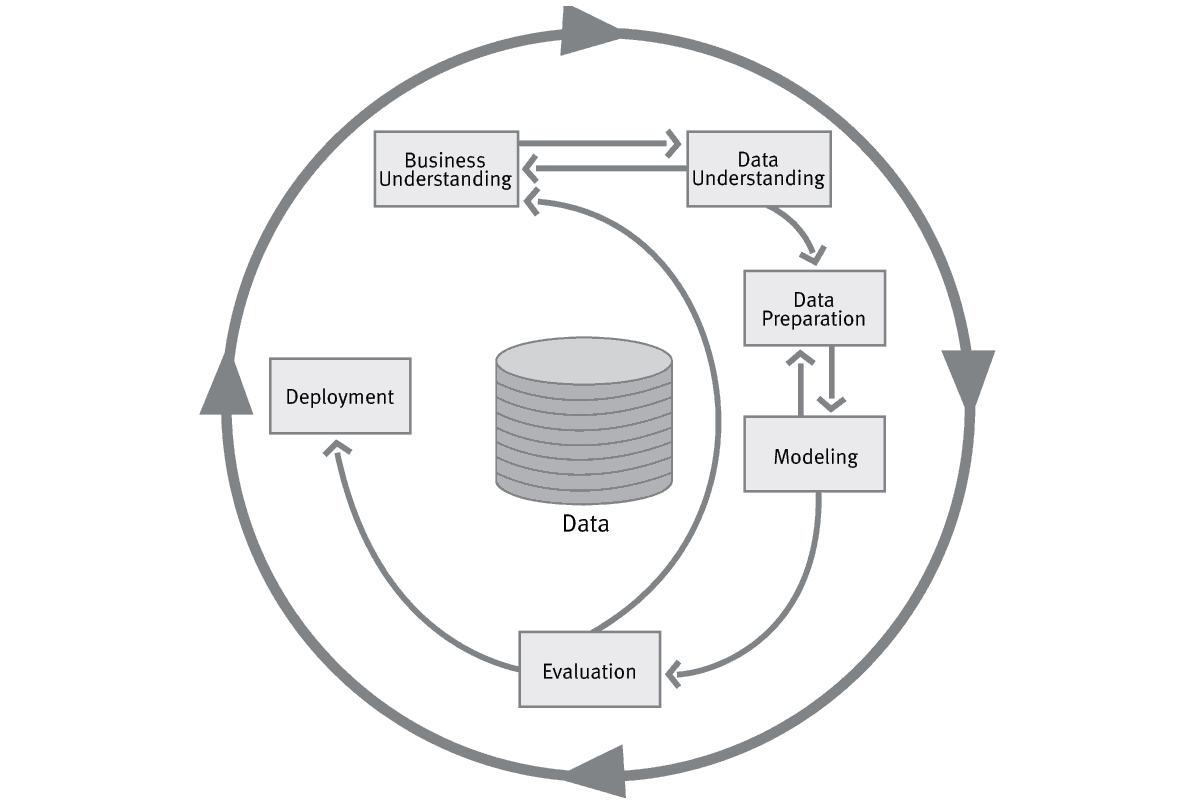
\includegraphics[scale=0.16]{./img/CRISP-DM.png}
	\captionsetup{format=hang}
	\caption[Optionaler Kurztitel für das Abbildunggsverzeichnis]{\label{fig:test}Demo-Abbildung, um zu verdeutlichen, wie gleitende Objekte 
		gesetzt werden und wie entsprechend die Quelle zitiert wird. \\Quelle: \cite[][S. 223]{TD15}}
\end{figure}

\subsection{Mathematische Formeln}
Auch\index{mathematisch!Formel} mathematische Ausdrücke\index{mathematisch!Ausdruck} können mit \LaTeX~ sehr gut gesetzt werden, wie man anhand der 
Gleichungen\index{mathematisch!Gleichung} \vref{eqn:e1} und \vref{eqn:e2} sehen kann -- konsultieren Sie hierzu bitte entsprechende Dokumentationen, 
die Online zur Verfügung stehen.
\begin{equation}
\left|{\frac{1}{N}}\sum_{n=1}^N \gamma(u_n)-{\frac{1}{2\pi}}\int_0^{2\pi}\gamma(t){ d}t\right| \le {\frac{\varepsilon}{3}}.\\
\label{eqn:e1}\\[\linewidth]
\end{equation}

\begin{equation}
f(x)=x^2
\label{eqn:e2}
\end{equation}

\subsection{Algorithmen}
Algorithmen\index{Algorithmus} können als Pseudocodes dargestellt und referenziert werden, wie z.\,B. in Algorithmus \vref{alg:euclid} -- 
sogar bis auf Zeilennummern (siehe die \texttt{while}-Anweisung in Zeile \vref{alg:euclid:while}). Schauen Sie sich hierzu bitte das 
Paket \texttt{algorithmicx} an.

\begin{algorithm}[H]
\begin{algorithmic}[1]
\Procedure{Euclid}{$a,b$}\Comment{The g.c.d. of a and b}
   \State $r\gets a\bmod b$
   \While{$r\not=0$}\Comment{We have the answer if r is 0} \label{alg:euclid:while}
      \State $a\gets b$
      \State $b\gets r$
      \State $r\gets a\bmod b$
   \EndWhile\label{euclidendwhile}
   \State \textbf{return} $b$\Comment{The gcd is b}
\EndProcedure
\end{algorithmic}
\caption{Euklidischer Algorithmus}\label{alg:euclid}
\end{algorithm}

Im obigen Beispiel wird der Euklidische Algorithmus in Pseudocode dargestellt. 
% !TEX root =  master.tex
\chapter{Beispiel-Kapitel: Noch ein Kapitel}

blabla

\lstset{language=Python, 
        numbers=left, 
        numberstyle=\tiny, 
        captionpos=b,
        keywordstyle=\color{blue},
        commentstyle=\color{green},
        stringstyle=\color{red}
        }

        
\section{Abschnitt mit Coding}

Der folgende Quelltext wird auch im Quelltextverzeichnis\index{Quelltext} referenziert:

\begin{lstlisting}[caption={\texttt{PrintMovieDB.py}},captionpos=b]
import numpy as np  
import matplotlib.pyplot as plt  
import pandas as pd  
from apyori import apriori

movie_data = pd.read_csv('./movie_dataset.csv', header = None)
num_records = len(movie_data)
print(num_records)
\end{lstlisting}

\section{Noch ein Abschnitt mit Coding}
Blabla



% Fazit und Ausblick
% !TEX root =  master.tex
\chapter{Zusammenfassung}

Dieses Kapitel enthält die Zusammenfassung der Arbeit mit Fazit und Ausblick.

\section{Fazit}

...

\section{Ausblick}

...

% Anhänge
\initializeAppendix
% !TEX root =  master.tex
\chapter{Beispiel-Anhang: Testanhang}
Anh\"ange\index{Anhang} werden am Ende Ihrer Arbeit vor dem Literaturverzeichnis und dem Index eingef\"ugt.

\section{Abschnitt im Anhang}

Blabla

\section{Noch ein Abschnitt im Anhang}


% !TEX root =  master.tex
\chapter{Beispiel-Anhang: Noch ein Testanhang}
 Noch ein Testanhang


\cleardoublepage


\cftaddtitleline{toc}{chapter}{Literaturverzeichnis}{\thepage}
\initializeBibliography


\cftaddtitleline{toc}{chapter}{Index}{\thepage}
\printindex

\end{document}